\chapter{Resultados}
\label{resultados}

Neste capítulo apresentaremos os espectros de massa referentes aos \textit{clusters} de prata que caracterizam os resultados experimentais obtidos neste trabalho.

\section{Espectros de nanopartículas de prata}
\label{sec:producao_cluster}
Foram realizados quatro experimentos para obtenção dos espectros de prata. Para cada um foram obtidos os dados dos \textit{clusters} com e sem a incidência de luz ultra violeta. 

Os dados fornecidos pelo sistema de aquisição
fornece o tempo de voo das partículas e as intensidade dos picos, como pode ser visto na Figura \ref{fig:ex_dados_brutos}. Depois de adquirido, os dados são tratados de forma a minimizar os ruídos existentes, e é feita uma normalização pela eficiência do detector de corrente, uma vez que as partículas com menor massa são melhor detectadas do que as partículas de maiores massas. O mesmo espectro com o tratamento de dados realizado pode ser visto na \ref{fig:0105_ledoff_dados_tratados}.




\begin{figure}
  \centering  
  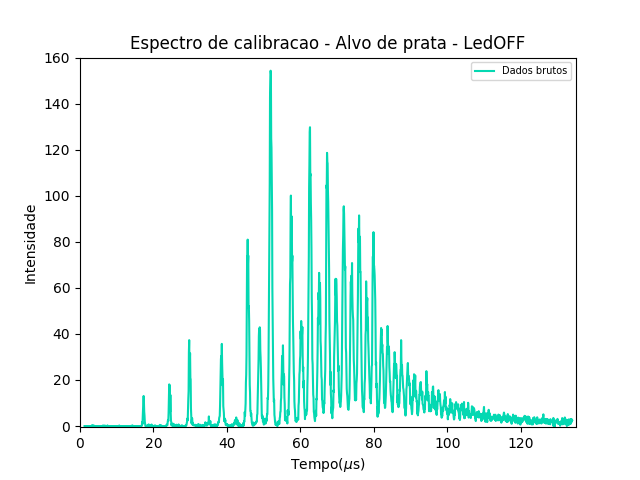
\includegraphics[width=0.7\textwidth]{graficos_resultados/0105_LEDOFF_semtratamento_exemplo.png}
  \caption{Espectro de calibração sem tratamento de dados.}
  \label{fig:ex_dados_brutos} 
\end{figure}

\begin{figure}
  \centering  
  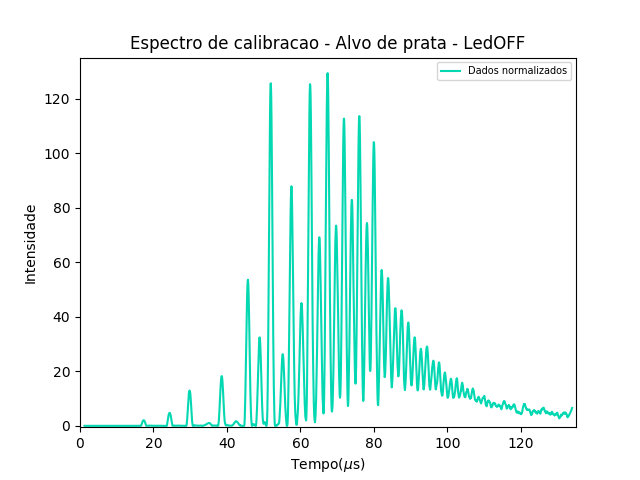
\includegraphics[width=0.7\textwidth]{graficos_resultados/0105_LEDOFF_normalizado_mcp.png}
  \caption{Espectro de calibração com tratamento de dados.}
  \label{fig:0105_ledoff_dados_tratados} 
\end{figure}

Para indicar quais são os picos presentes nos espectros, e assim encontrar as indicações do número de prata ($Ag_{1},Ag_{2},Ag_{3}...$), é necessário fazer uma calibração, onde são relacionadas o tempo de voo de cada partícula com as massas das próprias de forma a obter uma tendência quadrática, como veremos a seguir.

Com o objetivo de obter uma maior precisão na determinação dos tempos de voo das partículas de prata, é traçado uma curva gaussiana em cima de cada pico do espectro.

A Tabela \ref{tab:picos_encontados} mostra os valores dos picos encontrados, em comparação com os valores dos picos calculados teoricamente pela Equação \ref{eq:relacao_massa_tempo}. Dentro de uma certa tolerância é possível perceber que os picos encontrados correspondem com os que eram esperados. \textcolor{red}{barra de erro nos dados}

Sabendo o número de átomos de prata que corresponde a cada tempo de voo, é possível montar uma curva de calibração Massa $\times$ tempo, e assim realizar uma ajuste de uma curva quadrática para termos coeficientes que vão permitir identificar a massa de todo o espectro adquirido. O ajuste do espectro em questão pode ser vista na Figura \ref{fig:1105_curva_calib_ledoff}. As calibrações dos demais espectros serão apresentadas no Apêndice deste trabalho.

\begin{figure}
  \centering  
  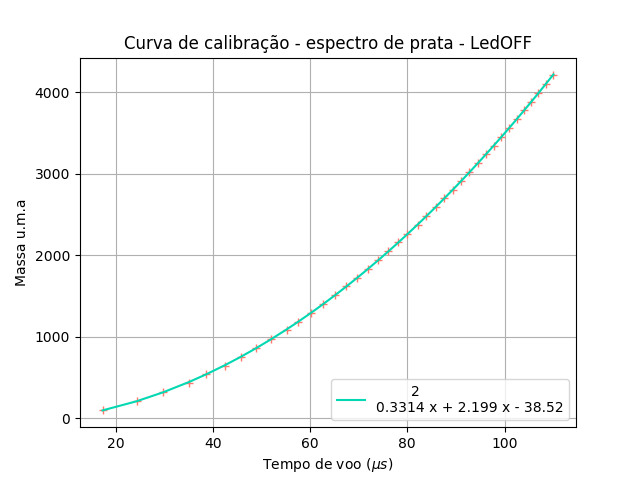
\includegraphics[width=0.7\textwidth]{graficos_resultados/0105_LEDOFF_curv_calib.png}
  \caption{Curva de calibração.}
  \label{fig:1105_curva_calib_ledoff} 
\end{figure}


\textcolor{red}{Precisa explicar que é massa/carga}




\begin{equation}
\label{eq:0105_polinomio_calib_ledoff}
M = 0,3187e^{2} t^2 + 2,525 t - 40,18
\end{equation}

Utilizando a Equação \ref{eq:0105_polinomio_calib_ledoff} é possível mudar o eixo de tempo de voo, da aquisição de dados, para o seu valor corresponde em massa, conforme do gráfico da Figura \ref{fig:0105_LEDOFF_espec_calib_ag_massa}.

\begin{figure}
  \centering  
  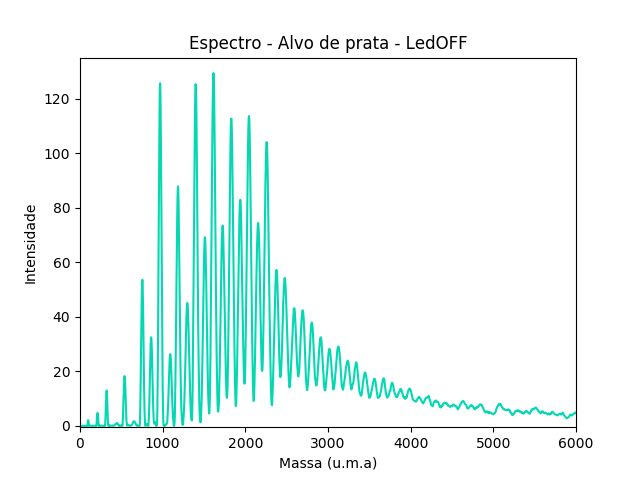
\includegraphics[width=0.7\textwidth]{graficos_resultados/0105_LEDOFF_espec_calib_ag_massa}
  \caption{Espectro de prata plotado na forma de intensidade por massa em unidade de massa atômica.}
  \label{fig:0105_LEDOFF_espec_calib_ag_massa} 
\end{figure}

\begin{table}
\centering
\caption{I- Tempo de voo dos átomos de Prata}
\label{tab:picos_encontados_01}
\begin{tabular}{|c|c|c|c|c|c|c|}
\hline
\begin{tabular}[c]{@{}c@{}}Prata\\ (N)\end{tabular} & \begin{tabular}[c]{@{}c@{}}Massa\\ teórica\\ (u.m.a)\end{tabular} & \begin{tabular}[c]{@{}c@{}}LED OFF\\ Massa\\ calculada\\ $\pm \Delta m$\\ (u.m.a)\end{tabular} & \begin{tabular}[c]{@{}c@{}}LED ON\\ Massa\\ calculada\\ $\pm \Delta m$\\ (u.m.a)\end{tabular} & \begin{tabular}[c]{@{}c@{}}Tempo\\ teórico\\ ($\mu s$)\end{tabular} & \begin{tabular}[c]{@{}c@{}}LED OFF\\ Tempo\\ calculado\\ $\pm \Delta t$\\ ($\mu s$)\end{tabular} & \begin{tabular}[c]{@{}c@{}}LED ON\\ Tempo\\ calculado\\ $\pm \Delta t$\\ ($\mu s$)\end{tabular} \\ \hline 
1&107.86&104$\pm$25&106$\pm$26&17.30&17$\pm$2&17$\pm$2\\ \hline 
2&215.72&215$\pm$35&215$\pm$35&24.47&24$\pm$2&24$\pm$2\\ \hline 
3&323.58&322$\pm$42&324$\pm$42&29.96&30$\pm$2&30$\pm$2\\ \hline 
4&431.44&438$\pm$49&433$\pm$48&34.60&35$\pm$2&34$\pm$2\\ \hline 
5&539.30&536$\pm$54&538$\pm$54&38.68&38$\pm$2&38$\pm$2\\ \hline 
6&647.16&652$\pm$59&650$\pm$59&42.38&42$\pm$2&42$\pm$2\\ \hline 
7&755.02&756$\pm$64&756$\pm$63&45.77&46$\pm$2&46$\pm$2\\ \hline 
8&862.88&857$\pm$68&859$\pm$68&48.93&49$\pm$2&49$\pm$2\\ \hline 
9&970.74&966$\pm$72&968$\pm$72&51.90&52$\pm$2&52$\pm$2\\ \hline 
10&1078.60&1092$\pm$76&1087$\pm$76&54.71&55$\pm$2&55$\pm$2\\ \hline 
11&1186.46&1179$\pm$79&1180$\pm$79&57.38&58$\pm$2&58$\pm$2\\ \hline 
12&1294.32&1293$\pm$83&1291$\pm$83&59.93&60$\pm$2&60$\pm$2\\ \hline 
13&1402.18&1399$\pm$86&1400$\pm$86&62.38&63$\pm$2&63$\pm$2\\ \hline 
14&1510.04&1512$\pm$90&1509$\pm$89&64.73&65$\pm$2&65$\pm$2\\ \hline 
15&1617.90&1614$\pm$93&1618$\pm$92&67.00&68$\pm$2&68$\pm$2\\ \hline 
16&1725.76&1720$\pm$95&1728$\pm$95&69.20&70$\pm$2&70$\pm$2\\ \hline 
17&1833.62&1829$\pm$98&1833$\pm$98&71.33&72$\pm$2&72$\pm$2\\ \hline 
18&1941.48&1938$\pm$101&1941$\pm$101&73.40&74$\pm$2&74$\pm$2\\ \hline 
19&2049.34&2053$\pm$104&2048$\pm$104&75.41&77$\pm$2&76$\pm$2\\ \hline 
20&2157.20&2164$\pm$107&2158$\pm$107&77.37&79$\pm$2&79$\pm$2\\ \hline 
\end{tabular} 
\end{table} 



